\documentclass{paper}
\usepackage{amssymb}
\usepackage{amsmath}
\usepackage{listings}
\usepackage{graphicx}
\usepackage{float}



\begin{document}

%\author{ Timothy Schwieg}
%\title{ Problem Set 2 }

%\maketitle
\section*{ Problem Set 2 }
Timothy Schwieg
\section*{ Design Document}
This python code should be able to take as an input, data collected from a Log-Series distribution. From that it should calculate the sample mean, and apply Newton's Method to calculate the zero of the log of the likelihood function. As an output it should return the Maximum Likelihood Estimator for $\theta$.

\section*{Flowchart}
\begin{figure}[H]
\centering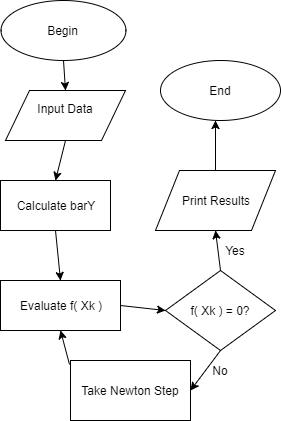
\includegraphics[height=1\textwidth]{FlowChart.png}
\caption{Program Flow}
\end{figure}

\section*{Test Data}
Test Data was generated by sampling from the Log-Series distribution with several different values of $\theta$. As edge cases, $\theta$ = .01 was used, but no edge case near 1 will be used because the code will fail. In realizations of the distribution where the number of entries in the final bin is large, $\bar{y}$ is an underestimate of the sample mean, as it assumes all the values are 9. However, using any weighted average instead of nine is making an assumption about $\theta$ whose estimation is the purpose of this code. This Code must simply be used with the awareness that it is not effective for realizations of the distribution with $\theta$ near 1. The Test Data was generated using theta = $\{ 0.01, .1, .2, .3, .4, .5, .6, .7, .8 \}$  The data was generated in R using the following code: 

\begin{lstlisting}[language=R]
theta <- c( 0.01, .1, .2, .3, .4, .5, .6, .7, .8 )
numSamples <- 1000

set.seed( 235711 )

for( j in 1:9 ) {

	realizations <- numeric( numSamples )
	probGenerator <- numeric( 9 )
	
	for( i in 1:8 ){
		probGenerator[i] <- ( (- theta[j]^i) / ( i*log( 1 - theta[j] ) ) )
	}
	
	#This gives us an option for 9+
	probGenerator[9] <- 1 - sum( probGenerator[1:8] )
	
	#I guess this is the discrete version of the inverse distribution applied to the Uniform
	simulations <- runif( numSamples )
	for( i in 1:numSamples ){
		realized <- 1
		while( simulations[i] > sum( probGenerator[1:realized] ) )
			realized <- realized + 1
		realizations[i] <- realized 
	}
	freqTable <- numeric( 9 )
	for( i in 1:9 )
		freqTable[i] <- sum( realizations == i )
		

	write(toString(freqTable),file="output.txt",append=TRUE)
	
}



\end{lstlisting}

This yielded the following result:
\begin{lstlisting}
994, 6, 0, 0, 0, 0, 0, 0, 0
948, 50, 2, 0, 0, 0, 0, 0, 0
893, 92, 14, 1, 0, 0, 0, 0, 0
843, 116, 33, 5, 3, 0, 0, 0, 0
792, 153, 36, 12, 3, 3, 1, 0, 0
706, 196, 63, 18, 8, 8, 0, 1, 0
663, 203, 76, 29, 10, 11, 5, 1, 2
568, 194, 112, 46, 32, 15, 19, 7, 7
513, 177, 103, 82, 30, 26, 22, 10, 37
\end{lstlisting}

It is worth noting that for this test data, convergence was not reached for the final data set, which contained 37 elements in the final bin. This appeared to be enough to understate $\bar{y}$ and consistently overstate our estimate: $x_k$. While censoring will not create a problem for the current assignment, it is worth noting that a different solution would be needed if this code were to be made for production. 

\section*{a.}

$f( \theta ) = \bar{y} + \frac{ \theta }{( 1 - \theta) log( 1 - \theta )}$

Let $\hat{ \theta }$ be the solution to $f( \theta ) = 0$. 

\section*{b.}
Note that: $f'( \theta ) = \frac{ \theta + log( 1 - \theta ) } { ( 1 - \theta )^2 log( 1 - \theta )^2 }$ The denominator is strictly positive, and the sign of $f'( \theta )$ is determined solely by the sign of $x + log( 1 - \theta )$.
\newline
Consider the Taylor polynomial of $log( 1 - \theta )$ centered around zero, with degree one, using Lagrange's Remainder Theorem. $$\frac{d}{d \theta} log( 1 - \theta ) = \frac{ -1 }{ 1 - \theta }$$
$$\frac{ d^2 }{ d^2 \theta } log( 1 - \theta ) = \frac{ -1 }{ (1 - \theta)^2 }$$
So: $log( 1 - \theta ) = -\theta - \frac{1}{2} c^2 \text{ where } c \in (0, \theta ).$ 
\newline
Thus: $x + log( 1 - \theta ) = - \frac{1}{2} c^2 \text{ where } c \in (0, \theta ).$ Note that this quantity is always negative. We can see now that $f'( \theta ) < 0 \forall \theta \in (0,1).$
Since $f( \theta )$ is strictly decreasing, it is one-to-one, and $\forall a,b \in \rm I\!R$ if $f(a) = f(b)$ then $a = b$. This implies any zero of the function must be unique. 

\section*{c.}
In order to solve for the zero of $f( \theta )$ Newton's Method will be applied to the problem. Each step of the problem will take the form: $$x_{k+1} = x_k - \frac{ f( x_k ) }{ f'( x_k ) } = x_k - \frac{ \bar{y} + \frac{ x_k }{ ( 1 - x_k ) log( 1 - x_k ) }}{ \frac{ x_k + log( 1 - x_k ) }{( 1 - x_k)^2 log( 1 - x_k )^2}} = \frac{ ( 1 - x_k)^2 log( 1 - x_k )^2 \bar{y} + x_k ( 1 - x_k ) log( 1 - x_k ) }{  x_k + log( 1 - x_k ) }$$


The python Code used to calculate the optimal is: 
\begin{lstlisting}[language=python]
import math

#This is f( theta ) 
def LogLikelihood( barY, theta ):
	"""Returns the LogLikelihood Function ( f( theta ) ) evaluated at barY and theta"""
	return barY  + ( theta ) / ( (1 - theta )*math.log( 1 - theta ) )


#This is the newton step taken as calculated in part c.
def NewtonStep( barY, Xk ):
	"""Returns the next step in Newton's method based for the zero of the logLikelihood function based on sample mean and Current step Xk"""
	return Xk - ( (1 - Xk )*(1 - Xk) * math.log( 1 - Xk )*math.log( 1 - Xk ) * barY + Xk*(1-Xk)*math.log( 1 - Xk) ) / ( Xk + math.log( 1 - Xk ) )
	
def ProblemSetTwo():
	"""This completes the requirements for Problem Set Two, namely reading a file containing realizations from a log series distribution and calculates the Maximum Likelihood Estimator"""
	#I am assuming the data is being fed in the form of frequencies only, comma seperated, beginning from 1 and going to 9+
	dataFile = open( "hw2Data.txt", "r" )
	storedData = dataFile.read().strip()
	dataFile.close()
	print( storedData )
	freqs = list( map( float, storedData.strip().split(',') ) )
	print( freqs)
	
	#We need this calculated from the start so we can avoid smearing
	
	sum = 0
	for i in range( 0, 9 ):
		sum += freqs[i]
	
	barY = 0
	#Remember to calculate the BarY that is least smeared
	#Note that we have assumed that the 9+ measurement was 9.
	#Maybe it would be better to weight it against the pmf of the Log-Series to get a weighted average of all the possibilities
	for i in range( 9 ):
		#Note that since python is 0 indexed and we are 1 indexed we add one to i
		barY += ( float(i+1) * freqs[i] / float(sum) )
		
	
	#We don't really have any reason to believe that this is a good starting position, however since we're dealing with a GLM problem, we should still converge quickly
	hatTheta = .5
	iterations = 0
	
	#Check for f( X_k ) = 0, and include a timeout counter in case something when wrong
	#Clamp it, because we are assuming all measurements at 9+ are 9, for high values of theta we will have problems with Newton's Method
	#This Clamp does not fix the problem, just prevents us from passing a negative number into log. This is a fault of us binning, and if we were to use a weighted average,
	#we would be making an assumption about theta, which is exactly the thing we are trying to estimate.
	while( abs( LogLikelihood( barY, hatTheta ) ) > .000001 and iterations < 10 ):
		hatTheta = max( min( NewtonStep( barY, hatTheta ), .99999999 ), 0.00000001 )
		iterations += 1
		
		

	#print( iterations )
	print( hatTheta )
	#print( LogLikelihood( barY, hatTheta ) )
	return

ProblemSetTwo()

700,205,50,26,10,6,1,1,1
[700.0, 205.0, 50.0, 26.0, 10.0, 6.0, 1.0, 1.0, 1.0]
0.5188415492137765

\end{lstlisting}

Using the python scrpt, the calculated value for $\hat{\theta}$ is 0.5188415492137765

\end{document}
